\chapter{Konkurenční aplikace}
\label{chap:competitive-apps}

Po prozkoumání podobného žánru her
(kooperace, komunikace a~rychlost reakcí)
dostupných v~obchodě Google Play,
byly vybrány konkurenční herní aplikace.
Tyto hry byly vybrány zejména podle popularity,
počtu stažení aplikace v~obchodě
a~podle subjektivně vnímaného potenciálu,
který má daná hra k~inspiraci pro tvorbu herní aplikace.

V~následujících podkapitolách jsou popsány vybrané čtyři konkurenční aplikace.
U~každé aplikace jsou také popsány klady a~zápory.

\section{DUAL!}

\begin{figure}[ht!]
    \centering
    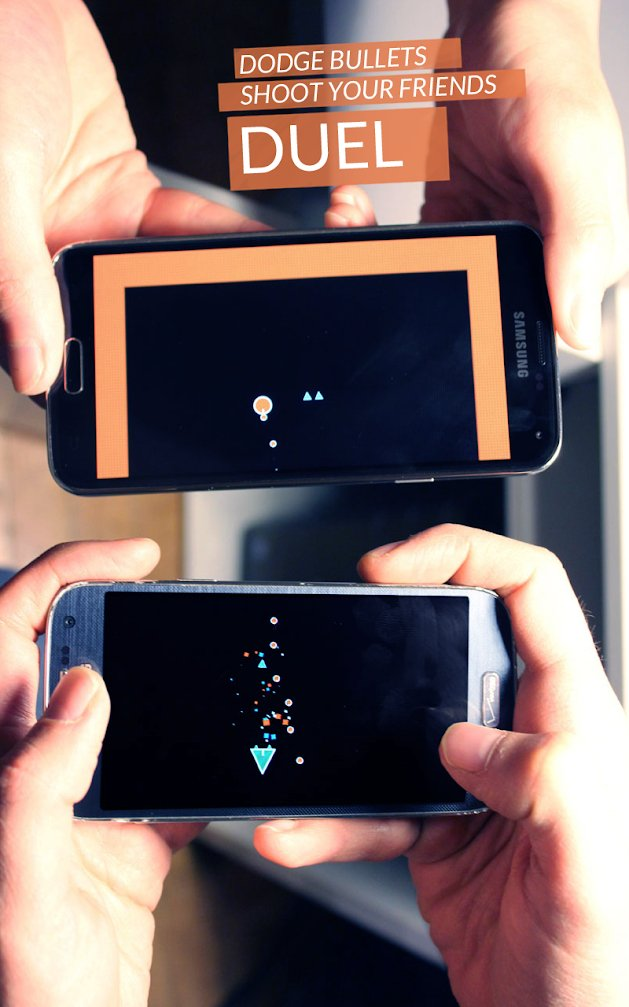
\includegraphics[width=0.5\linewidth]{assets/competitive-apps/dual.jpg}
    \caption{Screenshot hry DUAL! \cite{seabaa_dual}}
    \label{fig:dual}
\end{figure}

První vybranou hrou je \emph{DUAL!}.
Tato hra využívá zejména prvky kooperace a rychlosti reakcí
a je velmi akčně laděná.
Jak říká první věta stránky hry v obchodě Google Play:
\emph{\uv{Mezi lidmi, napříč obrazovkami.}} \cite{seabaa_dual} (překlad vlastní)

Hra má několik módů.
Jedním z módů je mód \uv{DUEL}, ve kterém dva hráči
--- každý na svém zařízení ---
bojují proti sobě.
Hra obsahuje další 2 módy, které však nejsou přístupní zdarma,
proto zde nebudou zohledněny a popsány.

Herní plocha je rozdělena do dvou 2D částí.
Každý hráč se může pohybovat pouze ve své části, na svém zařízení.
Herní postava hráče se ovládá natáčením jeho displeje.
Postava má zásobník střel a po klepnutí na plochu postava vystřelí.
Při podržení se postupně ze zásobníku nabíjí střely
a vystřelí se větší, ale trochu pomalejší, střela.
Rychlým použitím gesta švihnutí se postava otočí.
Pokud hráč vystřelí na své ploše,
střela za chvíli doletí do protihráčovi části.
Střele protihráče se dá buď takticky vyhnout,
nebo zneškodnit vystřelením vlastní střely.

Cílem hry je několikrát zasáhnout protihráče, a tím ho zneškodnit.
Po ukončení hry je možné v dané relaci s protihráčem začít další kolo hry.

\subsection*{Klady}

\begin{itemize}
    \item UI je velmi jednoduché, avšak přívětivé svými barvami a srozumitelností.
    \item Hra je velmi krátká a dá se mnohokrát opakovat.
\end{itemize}

\subsection*{Zápory}

\begin{itemize}
    \item K dispozici zdarma je pouze jeden herní mód.
    \item Nejsou dostupné žádné speciální funkce, které by hru obohatily.
\end{itemize}

\section{Sea Battle 2}

\begin{figure}
    \centering
    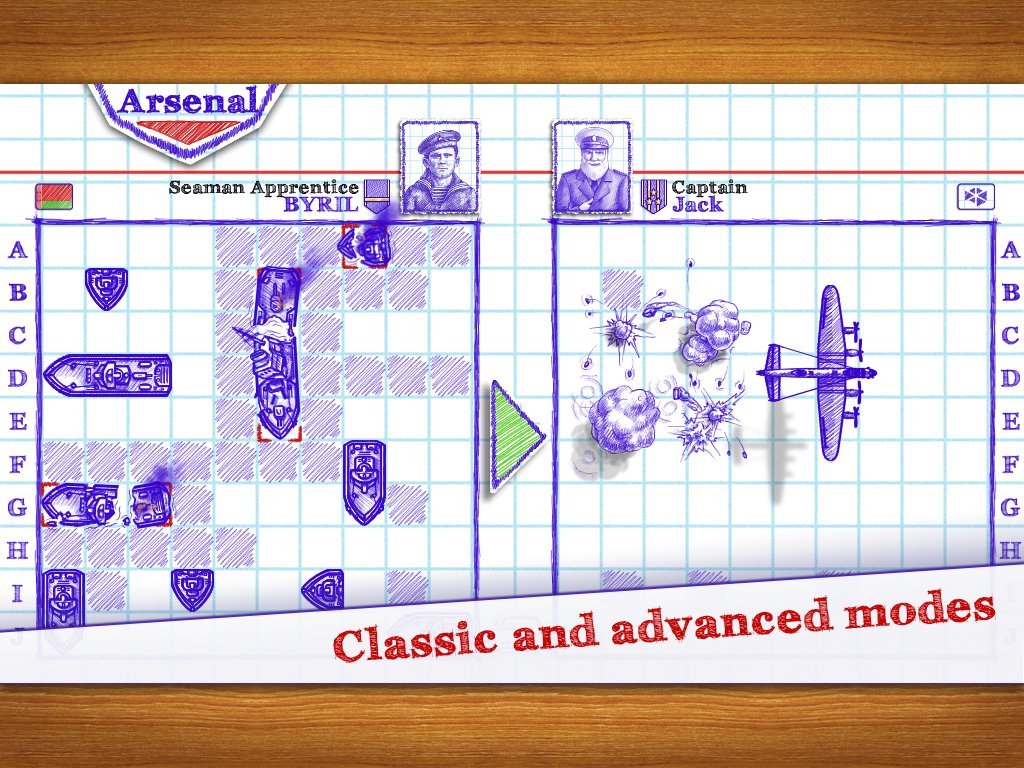
\includegraphics[width=0.5\linewidth]{assets/competitive-apps/sea-battle.jpg}
    \caption{Screenshot hry Sea Battle 2~\cite{byril_sea_battle_2}}
    \label{fig:sea-battle}
\end{figure}

Hra \emph{Sea Battle 2} sice není postavena na kooperaci a komunikaci mezi
hráči,
ale představuje hezkou reprezentaci klasické stolní hry v moderním pojetí.
Hráči z celého světa mezi sebou na svých zařízeních vedou souboje
a za každé vítězství postupně postupují v námořních
hodnostech.~\cite{byril_sea_battle_2}

Herní plocha obsahuje $10 \times 10$ políček,
kam si hráč rozloží své lodě.
Vedle toho jsou postupně vyobrazovány políčka protihráče.
UI je lazeno do podoby čtverečkovaného papíru s ručně kreslenými prvky.

Cílem hry, stejně jako v klasické stolní hře,
je zneškodnit všechny protivníkovy lodě.
Toho lze docílit klasicky pomocí bombardování,
nebo v pokročilém módu pomocí nejrůznějších letadel a pokročilých děl.
Pokročilý mód hezky rozšiřuje hru o nové strategie,
čímž činí hru zajímavější.

\subsection*{Klady}

\begin{itemize}
    \item Známý koncept hry.
    \item Obohacení hry s pokročilým módem o nové prvky.
\end{itemize}

\subsection*{Zápory}

\begin{itemize}
    \item UI nepůsobí přívětivě.
    \item UI nelze přibližovat,
    což způsobuje problémy s dotyky na jednotlivá políčka.
\end{itemize}

\section{Keep Talking and Nobody Explodes}

\begin{figure}
    \centering
    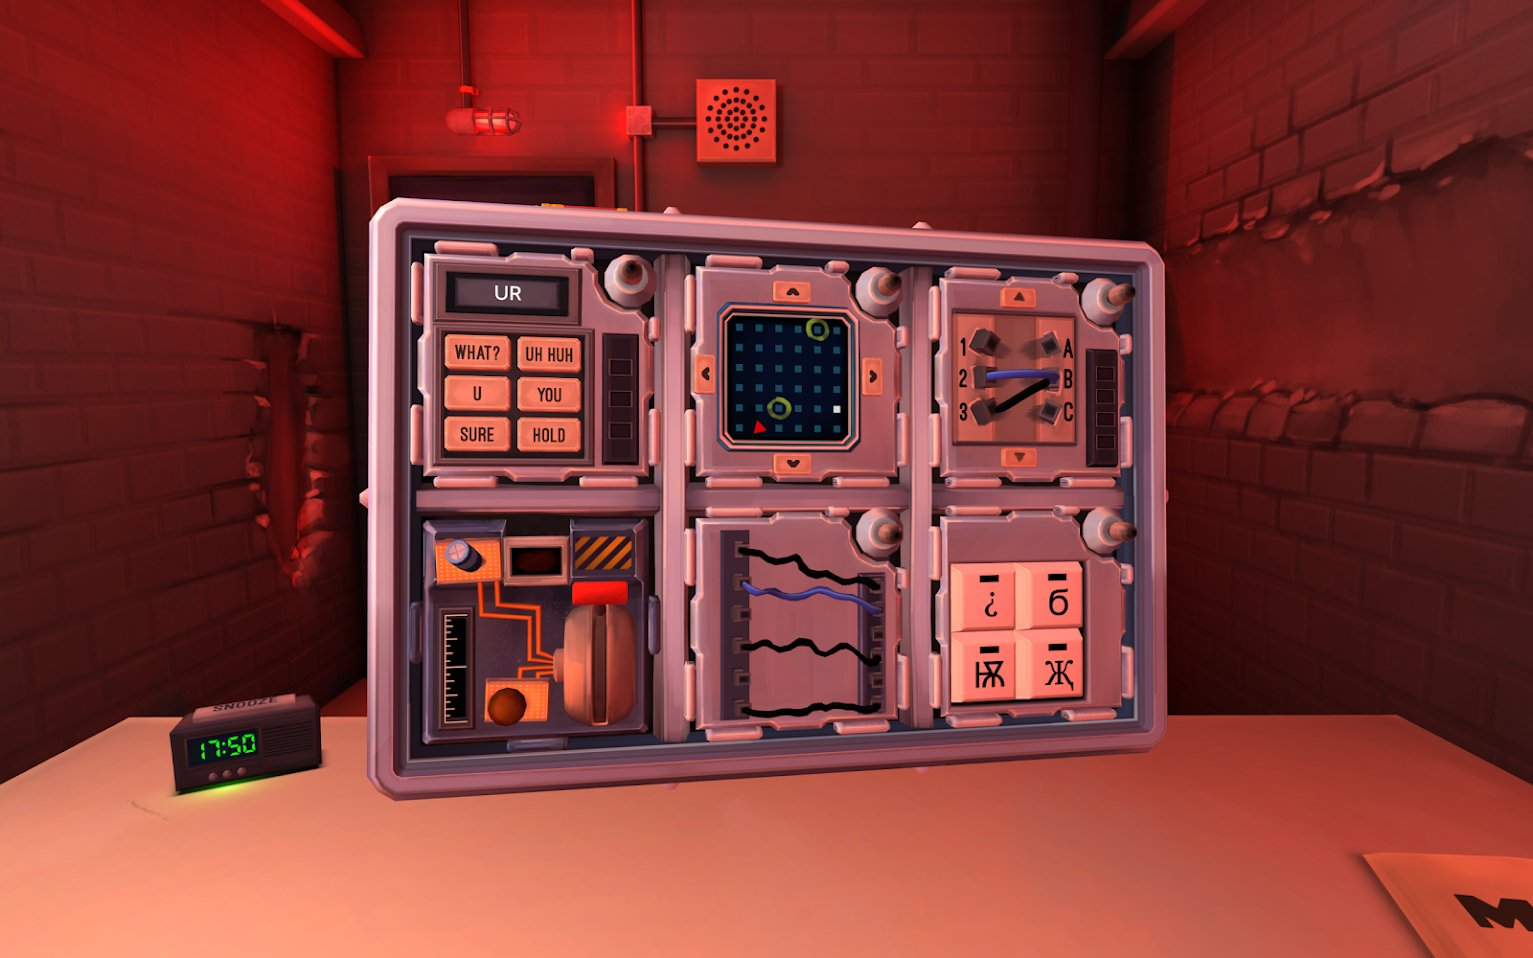
\includegraphics[width=0.5\linewidth]{assets/competitive-apps/keep-talking.jpg}
    \caption{Screenshot hry Keep Talking and Nobody Explodes~\cite{steelcrategamesinc_keep_talking}}
    \label{fig:keep-talking}
\end{figure}

Ve hře \emph{Keep Talking and Nobody Explodes} závisí všechno na správné
kooperaci a komunikaci.
Tato velmi oceňovaná hra existuje ve verzi pro desktop, konzole,
virtuální realitu i mobily.~\cite{steelcrategamesinc_keep_talking}

Hra má předpřipravená herní kola s daným typem bomby.
Bomba je koncipována jako kufřík s několika moduly a časomírou,
která se nebezpečně rychle odpočítává.
Jeden hráč vidí bombu.
Další hráč, případně skupina hráčů, mají k dispozici manuál s instrukcemi.
Manuál mohou prohlížet jak v elektronické, tak i v papírové podobě.
Manuál je totiž pro všechny hry shodný.

Veškerá komunikace probíhá pouze slovně.
Hráč s bombou tak nahlásí hráči s manuálem například to,
že vidí červené tlačítko s textem \uv{defuse}.
Druhý hráč pak v manuálu vyhledá daný modul tlačítka, řídí se instrukcemi a
podstatné informace k zneškodnění předá prvnímu hráči.

Cíl každého kola je zneškodnění bomby.
Důraz je také kladen na čas zneškodnění a počet udělaných chyb.
Po skončení kola může hráč porovnat svůj výsledek s ostatními hráči v žebříčku.

\subsection*{Klady}

\begin{itemize}
    \item UI je laděné jako pohled na stůl, na kterém je bomba a časomíra,
    což dodává hře atmostféru a vtáhne hráče do děje.
    \item Světla v místnosti blikají, případně se náhodně vypínají a zapínají.
    To přidává na efektu zejména v situácích,
    kdy zbývá už jen pár sekund a bomba není dobře vidět.
    \item Přestože je grafika jednodušší, samotná bomba je velmi přehledná.
    \item Manuál je stejný pro všechna herní kola. Lze jej tedy i vytisknout.
\end{itemize}

\subsection*{Zápory}

\begin{itemize}
    \item U složitějších modulů je manuál občas hůře pochopitelný.
\end{itemize}

\section{Spaceteam}

\begin{figure}
    \centering
    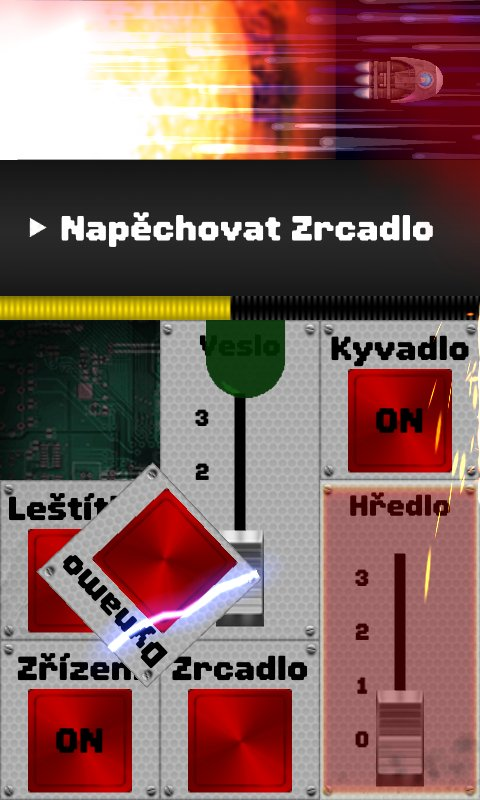
\includegraphics[width=0.5\linewidth]{assets/competitive-apps/spaceteam.jpg}
    \caption{Screenshot hry Spaceteam~\cite{henrysmithinc_spaceteam}}
    \label{fig:spaceteam}
\end{figure}

Poslední hra, \emph{Spaceteam}, si zakládá na rychlosti reakcí a velmi rychlé
komunikaci.
To shrnuje první věta na stránce hry v obchodě Google Play:
\emph{\uv{Mačkáš rád talčítka a řveš na své kamarády?
Jo? A i kdyby ne, zkus se na chvíli stát členem vesmírné posádky a zažij,
co to znamná být Spaceteam.}}
\cite{henrysmithinc_spaceteam}

Herní plocha je plná náhodných tlačítek, přepínačů, posouvátek a dalších věcí,
které dohromady tvoří ovládací prvky hry.
Každému hráči přichází postupně do zařízení série příkazů,
které cílí na určitou interakci s ovládacími prvky.

Hra je rozdělena na herní kola.
Každé herní kolo má vlastní množinu ovládacích prvků a příkazů.

Zapeklitost komunikace spočívá v tom,
že příkazy se netýkají pouze prvků na daném zařízení,
ale i prvků ze zařízení ostatních hráčů.
Některé příkazy také cílí na všechny hráče.
Příkladem takového příkazu je například zatřesení všemi zařízeními najednou.

Každý chybný krok je penalizován.
Penalizace se postupně projevuje například zhoršením přístupnosti k ovládacím
prvkům.
Cílem hry je dostat se přes co nejvíce herních kol.
Po skončení hry následuje shrnující statistika a ocenění jednotlivých hráčů.

\subsection*{Klady}

\begin{itemize}
    \item UI úvodní obrazovky a přihlašování do hry vypadá velmi efektně.
    \item Tlačítka i příkazy obsahují řadu technologických pojmů,
    což dodává hře na správné atmosféře.
    \item Finální ocenění hráčů působí vřelým dojmem.
\end{itemize}

\subsection*{Zápory}

\begin{itemize}
    \item Herní obrazovka má poněkud zastaralé, až nevkusné, prvky.
    \item Hra probíhá až příliš rychle.
    Nutno přiznat, že tento fakt není nutně nevýhoda,
    avšak ubírá to na prvku kvalitnější komunikace.
    \item Hra nemá možnost přihlášení,
    a tedy shromažďování a uchovávání statistik.
\end{itemize}


\section{Zhodnocení}

Aplikace vyvíjená v~rámci praktické práce je koncepčně podobná ke hrám
\emph{Spaceteam} a~\emph{Keep Talking and Nobody Explodes}.
Obě tyto hry pracují s~variací modulů,
které musí být nějakým způsobem splněny.
Zbylé dvě hry naopak pracují s~jiným stylem hry,
avšak také zachovávají prvky kooperace a~komunikace.
Ze všech her je vhodné se inspirovat jednoduchým UI a~krátkými hrami,
například v~podobě misí,
jelikož jde vidět,
že kratší hry mají velký úspěch,
zřejmě proto,
že je lze hrát kdykoli a~kdekoli.
Zároveň je velkým kladem všech zmíněných her příběh a~atmosféra,
zatímco se zdá,
že hezké UI nehraje příliš velkou roli
a~je tedy vhodnější zaměřit se na hratelnost samotnou.
Nevýhodou hry \emph{Spaceteam} je nemožnost přihlášení a~udržování statistik
napříč zařízeními.
Cílem je využít zmíněné klady a~zápory a~vhodně je zakomponovat do vyvíjené
aplikace.
